\newpage
\section{Simulation Analysis and Results Comparison}
\label{sec:simulation}

Here we will compare the theoretical results achieved by the method in the previous section to the ones obtained by simulating the chosen circuit in Ngspice. 

The first plots shown are of the variables $V_{in}$, $V_{o}$ and $V_{out}$ in function of time. Plot \ref{fig:gteo1} corresponds to the theoretical analysis and plot \ref{fig:gsim1} is the simulation one. The values for the ripple and deviation are in tables \ref{tab:tteo1} and \ref{tab:tsim1}.

%%%%???? O QUE POR AQUI NAO TENHO NADA NA PASTA NA PARTE DA SIM PQ DA ERRO

\begin{figure}[!ht] \centering
\caption{The theoretical values of $V_{in}$, $V_{o}$ and $V_{out}$ in function of time}
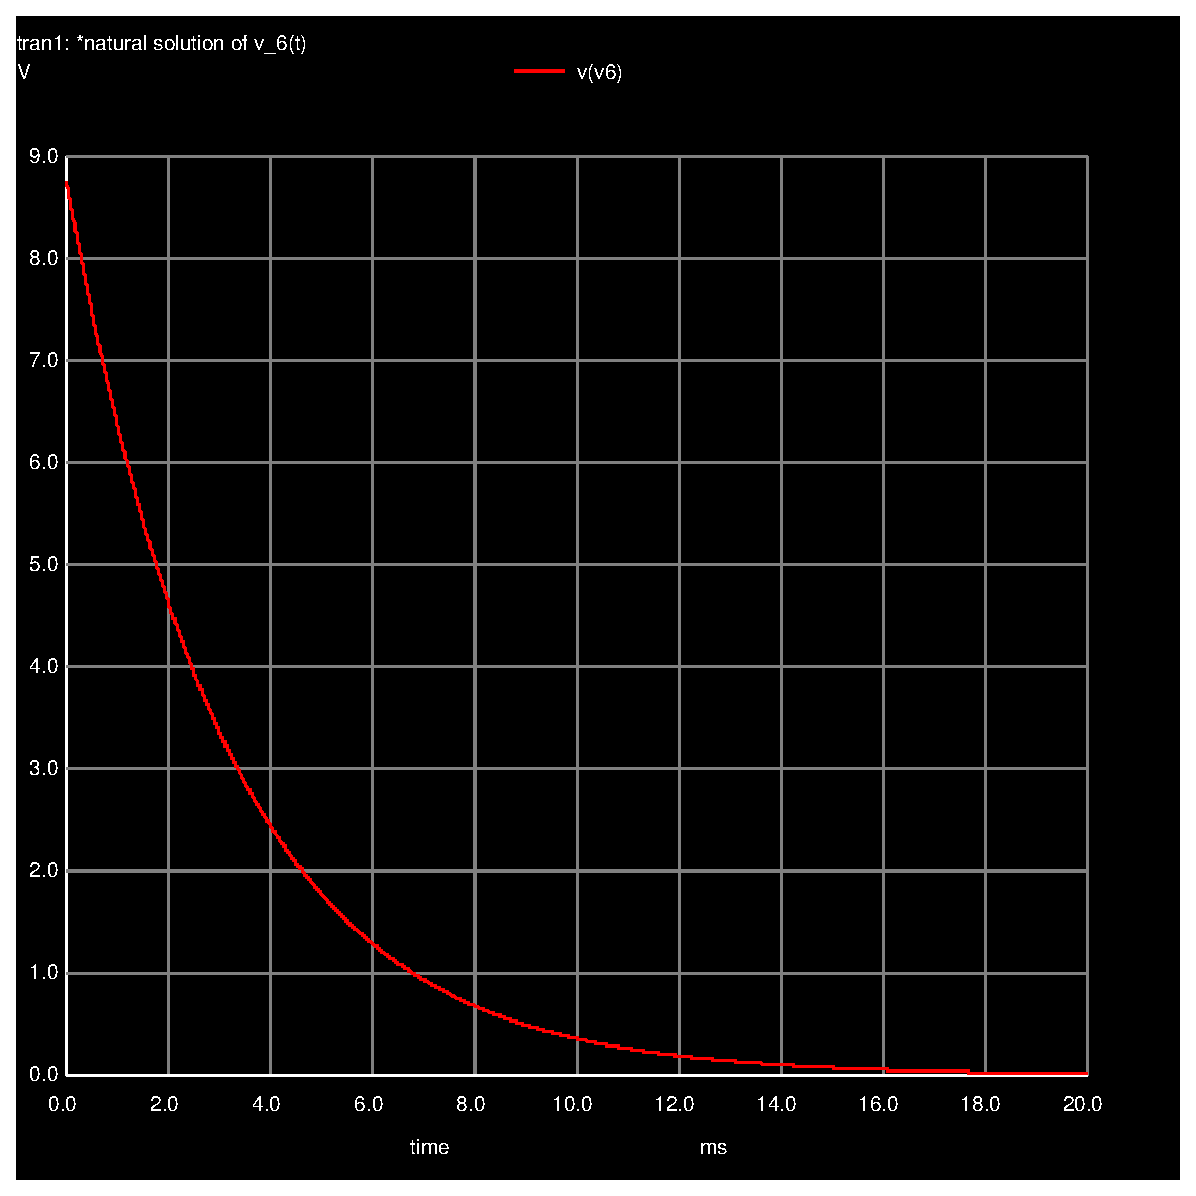
\includegraphics[width=0.6\linewidth]{trans3.eps}
\label{fig:gteo1}
\end{figure}
\newpage

\begin{table}[h]
    \centering
    \begin{tabular}{|l|c|}
    \hline
    {\bf Symbol} & {\bf Value [V]} \\ \hline
    \input{theo_table_del.tex} 
    \end{tabular}
    \caption{Theoretical Values for Ripple and Deviation.}
    \label{tab:tteo1}
\end{table}

\begin{figure}[!ht] \centering
\caption{The simulation values of $V_{in}$, $V_{o}$ and $V_{out}$ in function of time}
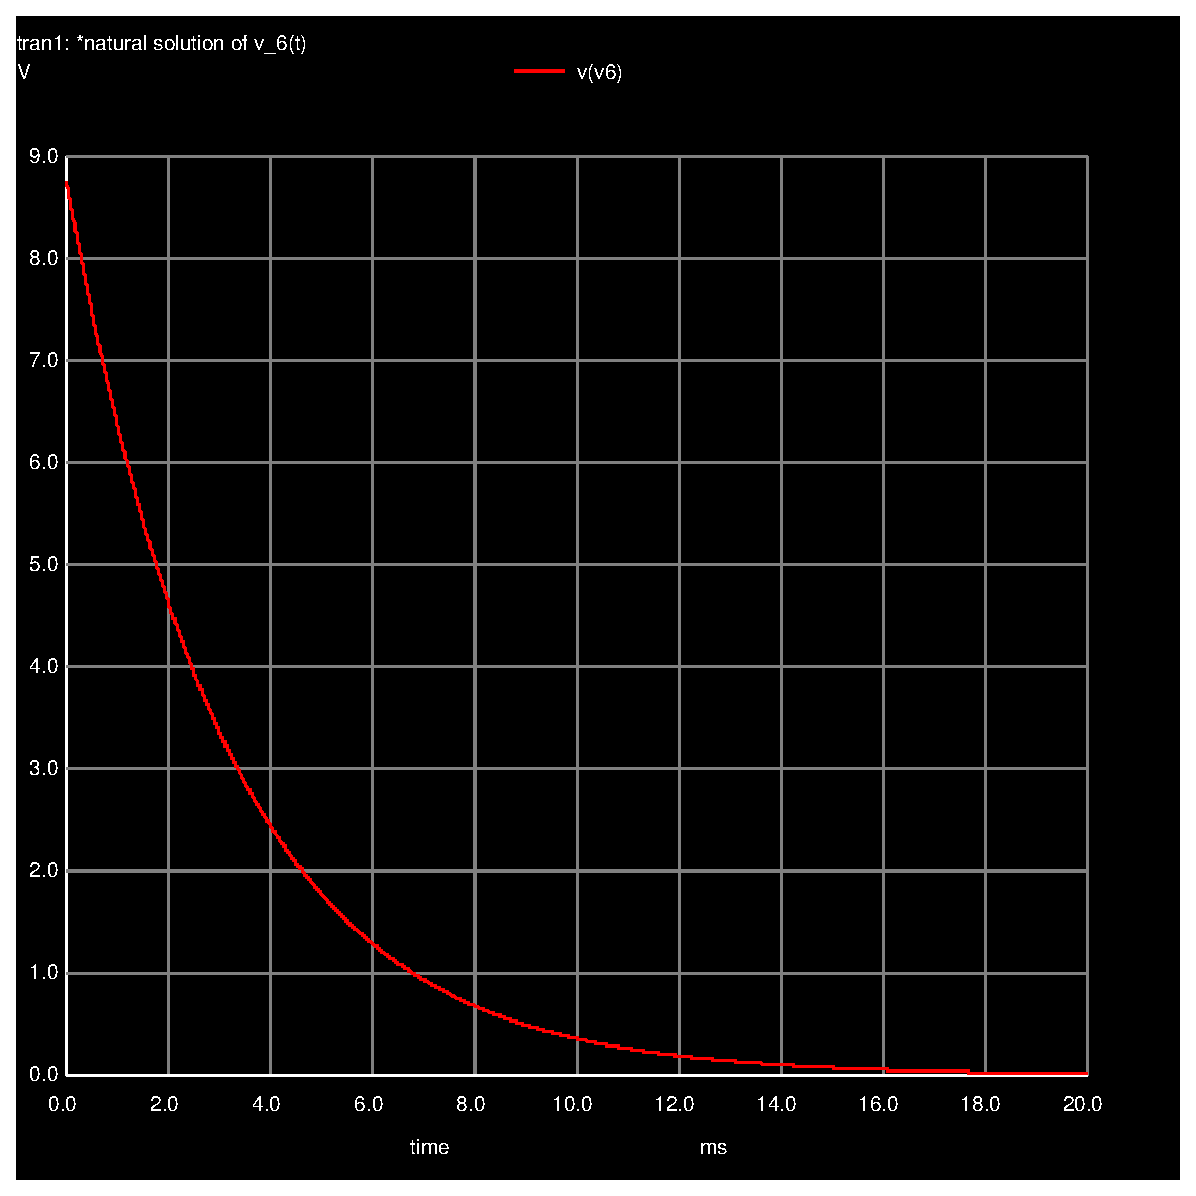
\includegraphics[width=0.6\linewidth]{trans3.eps}
\label{fig:gsim1}
\end{figure}
\newpage

\begin{table}[h]
    \centering
    \begin{tabular}{|l|c|}
    \hline
    {\bf Symbol} & {\bf Value [V]} \\ \hline
    \input{theo_table_del.tex} 
    \end{tabular}
    \caption{Simulation Values for Ripple and Deviation.}
    \label{tab:tsim1}
\end{table}







